\subsubsection{Squid}
\label{soa:tecnologias:squid}

Un \eng{proxy server}, también conocido como \eng{forward proxy server}, actúa como un proxy para los dispositivos que se conectan a él.  Una implementación típica puede ser un \eng{forward proxy} que provee acceso a internet a N clientes.
En cambio, un \eng{reverse proxy server} es un servidor proxy que recupera recursos desde uno o mas servidores.  Estos recursos se devuelven al cliente como si se hubieran originado desde el propio servidor, es decir, actúa como intermediario entre los clientes y servidores.  Los \eng{reverse proxys} se implementan en las proximidades de los \eng{web servers}, a veces realizan tareas como balanceo de carga, autenticación, o \eng{caching}.

\begin{figure}[H]
  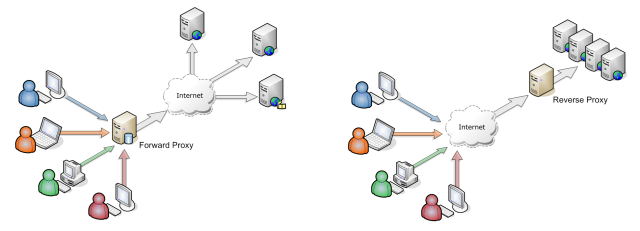
\includegraphics[width=\linewidth]{src/images/03-capitulo-3/tecnologias/squid/forward-reverse-proxy.png}
  \caption{Forward proxy y reverse proxy}
  \label{fig:varnish}
\end{figure}

\gls{db:squid} es un \eng{proxy server} (\eng{forward proxy server}) para la Web, soporta \gls{proto:http}, \gls{proto:https}, \gls{acro:ftp}, entre otros. Reduce el ancho de banda y mejora los tiempos de respuesta por el almacenamiento en caché y la reutilización de las páginas web frecuentemente solicitadas.  Puede implementarse en la mayoría de los sistemas operativos disponibles, incluyendo Windows y está disponible bajo licencia GNU GPL.

\gls{db:squid} es usado por cientos de proveedores de internet en todo el mundo, para proporcionar a sus usuarios el mejor acceso posible a la web.  Optimiza el flujo de datos entre el cliente y el servidor, utilizando el contenido en caches frecuentemente usado, ahorrando de esta manera ancho de banda y obteniendo mejoras en el rendimiento de los clientes.

ver RFC 2186: Internet Cache Protocol (ICP), version 2
ver http://www.ietf.org/rfc/rfc2186.txt


\paragraph{Licencia}

GNU General Public License

\paragraph{Instalación}

A continuación se detallan los pasos para instalar Squid en un servidor con Ubuntu 14.04.  Antes de comnenzar con la instación y configuración de Squid, debemos actualizar el software del servidor a su última versión:

\begin{listing}[H]
  \bashfile{src/03-capitulo-3/tecnologias/cache/code/squid/00-preparacion.sh}
  \caption{Actualización del sistema de base}
  \label{soa:tecnologias:squid-cache:bash-preparacion}
\end{listing}

Una vez que hemos terminado la actulización del equipo, estamos en condiciones de iniciar la instalación de Squid.  Squid se encuentra disponible en los repositorios de Ubuntu, para instalarlo en el servidor debemos ejecutar el siguiente comando:

\begin{listing}[H]
  \bashfile{src/03-capitulo-3/tecnologias/cache/code/squid/01-preparacion.sh}
  \caption{Instalación de Squid}
  \label{soa:tecnologias:squid-cache01:bash-preparacion}
\end{listing}

La configuración principal de Squid se encuentra en /etc/squid3/squid.conf.  Antes de realizar cualquier cambio en la configuración origincal, realizamos una copia del archivo.

\begin{listing}[H]
  \bashfile{src/03-capitulo-3/tecnologias/cache/code/squid/02-preparacion.sh}
  \caption{Copia de respando de configuración de Squid}
  \label{soa:tecnologias:squid-cache02:bash-preparacion}
\end{listing}

Editamos la configuración

\begin{listing}[H]
  \bashfile{src/03-capitulo-3/tecnologias/cache/code/squid/03-preparacion.sh}
  \caption{Configuración de Squid}
  \label{soa:tecnologias:squid-cache03:bash-preparacion}
\end{listing}

Lo primero que debemos configurar es el puerto en el que Squid estará escuchando las peticinas, por defecto, Squid escucha las peticioens en el puerto 3128.  Para cambiar el puerto por defecto, debemos editar la directiva \texttt{http\_port}.  En nuestro caso particular, configuramos el puerto 8888.

\begin{listing}[H]
  \bashfile{src/03-capitulo-3/tecnologias/cache/code/squid/04-preparacion.sh}
  \caption{Configuracón de puerto}
  \label{soa:tecnologias:squid-cache04:bash-preparacion}
\end{listing}

Por defecto, el servidor proxy HTTP no permite el acceso a nadie.  Para permitir el acceso al servidor desde cualquier IP, debemos editar la directiva \texttt{http\_access} de la siguiente manera:

\begin{listing}[H]
  \bashfile{src/03-capitulo-3/tecnologias/cache/code/squid/05-preparacion.sh}
  \caption{Configuración de acceso al servidor}
  \label{soa:tecnologias:squid-cache05:bash-preparacion}
\end{listing}

Una vez que hemos realizado las configuraciones necesarias, debemos guardar los cambios y reiniciar el servicio de Squid, para que tome los cambios.  Para reiniciar el servio ejecutamos el siguiente comando:

\begin{listing}[H]
  \bashfile{src/03-capitulo-3/tecnologias/cache/code/squid/06-preparacion.sh}
  \caption{Renicio del servicio Squid}
  \label{soa:tecnologias:squid-cache06:bash-preparacion}
\end{listing}

Para verificar el funcionamiento del servidor proxy, configuramos manualmente los datos de nuestro proxy en el navegador, ingresando la IP del servidor proxy y el puerto anteriomente configurado.
En caso de que tengamos problemas, podemos ver log access.log para obtener mas información:

\begin{listing}[H]
  \bashfile{src/03-capitulo-3/tecnologias/cache/code/squid/07-preparacion.sh}
  \caption{Verificación del funcionamiento de Squid}
  \label{soa:tecnologias:squid-cache07:bash-preparacion}
\end{listing}
